\documentclass[Afour,sageh,times]{sagej}
\usepackage{moreverb,url}

\usepackage[colorlinks,bookmarksopen,bookmarksnumbered,citecolor=red,urlcolor=red]{hyperref}

\usepackage{chngpage}

\newcommand\BibTeX{{\rmfamily B\kern-.05em \textsc{i\kern-.025em b}\kern-.08em
T\kern-.1667em\lower.7ex\hbox{E}\kern-.125emX}}

\def\volumeyear{2017}


\usepackage[utf8]{inputenc}
\usepackage[T1]{fontenc}

%%%%%
% variable to include comments or not in the compilation ; set to 1 to include
%\def \draft {1}
\def \draft {0}



\usepackage{xparse}
\usepackage{ifthen}

\DeclareDocumentCommand{\comment}{o m o o o o}
{\ifthenelse{\draft=1}{
  \IfValueT{#1}{
      \textcolor{red}{\textbf{C (#1) : }#2}
      \IfValueT{#3}{\textcolor{blue}{\textbf{A1 : }#3}}
      \IfValueT{#4}{\textcolor{ForestGreen}{\textbf{A2 : }#4}}
      \IfValueT{#5}{\textcolor{red!50!blue}{\textbf{A3 : }#5}}
      \IfValueT{#6}{\textcolor{Aquamarine}{\textbf{A4 : }#6}}
    }
    \IfNoValueT{#1}{
      \textcolor{red}{\textbf{C : }#2}
      \IfValueT{#3}{\textcolor{blue}{\textbf{A1 : }#3}}
      \IfValueT{#4}{\textcolor{ForestGreen}{\textbf{A2 : }#4}}
      \IfValueT{#5}{\textcolor{red!50!blue}{\textbf{A3 : }#5}}
      \IfValueT{#6}{\textcolor{Aquamarine}{\textbf{A4 : }#6}}
    }
 }{}
}




% todo
%\newcommand{\todo}[1]{
%\ifthenelse{\draft=1}{\textcolor{red!50!blue}{\textbf{TODO : \textit{#1}}}}{}
%}
\DeclareDocumentCommand{\todo}{o m}{
  \ifthenelse{\draft=1}{
    \IfValueT{#1}{\textcolor{red!50!blue}{\textbf{TODO (#1) : \textit{#2}}}}
    \IfNoValueT{#1}{\textcolor{red!50!blue}{\textbf{TODO : \textit{#2}}}}
  }{}
}

%\date{}
%\renewcommand\abstractname{\fontsize{14pt}{0}\textbf{Abstract}\selectfont}

%\usepackage[left=25mm, right=25mm, top=25mm, bottom=25mm, includehead=false, includefoot=false]{geometry}

%\usepackage{graphicx}
%\usepackage{url}
%\usepackage[round,semicolon]{natbib}  % Citation styles https://www.sharelatex.com/learn/Natbib_citation_styles
%\bibliographystyle{humannat}
%\renewcommand{\bibsection}{}
%\renewcommand{\bibhang}{\setlength{-1px}}


%\usepackage{authblk} % For author lists
%\renewcommand\Authfont{\fontsize{11}{1}\selectfont}
%\renewcommand\Affilfont{\fontsize{9}{1}\selectfont}

%\renewcommand*\footnoterule{}

\usepackage[table]{xcolor}
\usepackage[parfill]{parskip} % Line between paragraphs
\usepackage{amsmath}
%\pagenumbering{arabic} 

%\usepackage{sectsty}
%\allsectionsfont{\sffamily}

%\usepackage[pdftex]{hyperref} 
%\hypersetup{pdfborder={0 0 0} }


\usepackage[flushleft]{threeparttable}



%%%%%%%%%%%%%%%%%%%%%%%%%
%% -- from ecrc template
%%%%%%%%%%%%%%%%%%%%%%%%%


%% set the volume if you know. Otherwise `00'
\volume{00}

%% set the starting page if not 1
\firstpage{1}



\jid{}


\biboptions{authoryear}




\usepackage{soul}
\soulregister\cite7
\soulregister\citep7
\soulregister\ref7

%\usepackage[final]{changes}
\usepackage{changes}


\setaddedmarkup{\textcolor{black}{\hl{#1}}}
\setdeletedmarkup{\textcolor{red}{\sout{#1}}}

% add line number
\usepackage{lineno}
\linenumbers








\begin{document}

% **************  TITLE AND AUTHOR INFORMATION **************


\runninghead{Cottineau \& al.}


\title{Initial spatial conditions in simulation models: the missing leg of sensitivity analyses?}

\author{Cl{\' e}mentine Cottineau\affilnum{1}, Juste Raimbault\affilnum{2,4}, Marion Le Texier\affilnum{3}, Florent Le N{\' e}chet\affilnum{4}, Romain Reuillon\affilnum{2,5}
}

\affiliation{\affilnum{1}Centre for Advanced Spatial Analysis, University College London, UK\\
\affilnum{2}UMR 8504 G{\'e}ographie-cit{\'e}s, Paris, France\\
\affilnum{3}UMR 6266 IDEES, Universit{\'e} de Rouen Normandie, France\\
\affilnum{4}Laboratoire Ville Mobilit{\'e} Transport, Universit{\'e} Paris-Est, France\\
\affilnum{5}Institut des Syst{\`e}mes Complexes Paris Ile-de-France, France}

\corrauth{Corresponding author
address.}

\email{c.cottineau@ucl.ac.uk}



% **************  ABSTRACT  **************

\begin{abstract}
%\noindent
%\setlength{\parindent}{0pt}
Although simulation models of geographical systems in general and agent-based models in particular represent a fantastic opportunity to explore socio-spatial behaviours and to test a variety of scenarios for public policy, the validity of generative models is uncertain until their results are proven robust. Sensitivity analysis usually include the analysis of the effect of stochasticity on the variability of results, as well as the effects of small parameter changes. However, initial spatial conditions are usually taken for granted in geographical models, thus leaving completely unexplored the effect of spatial arrangements on the interaction of agents and of their interactions with the environment. In this contribution, we present a method to assess the effect of initial spatial conditions on simulation models, using a systematic generator controlled by meta-parameter to create density grids used in spatial simulation models. We show, with the example of two very classical agent-based models (Schelling's models of segregation and Sugarscape) that the effect of space in simulation is significant, and sometimes even larger than parameters themselves. We do so using high performance computing in a very simple and straightforward open-source workflow.
\end{abstract}

\keywords{Space, Initial conditions, Sensitivity, ABM}

\maketitle


% **************  MAIN BODY OF THE PAPER **************


%%%%%%%%%%%%%%%%%%%%%%
\section{Introduction}
%%%%%%%%%%%%%%%%%%%%%%

Simulation has been recognised and increasingly used by geographers to explore various geographical processes and problems within virtual laboratories. It appears as a very fruitful way to overcome the difficulty of analytic resolution of many spatial models developed in the past, and to explore the possible trajectories of social and ecological systems in space and time. The specificity of geographical models compared with models from other social sciences is usually regarded as the way geographers consider space and spatial interactions, driven by an explicit interest in the way space influences the outcomes of the model. Geographers are indeed concerned about understanding and modelling how space plays a role in social interactions and environmental processes, and whether its action is placed-based or place-neutral. We think simulation can become a very good tool to achieve this, provided that models include relevant spatial description and modelling, behavioural rules that take space into account, and provided model evaluation  stresses the sensitivity of output variations to the way space is modelled. This communication focuses on a way to do  so: by using a sensitivity method to test the model's outcomes to initial spatial conditions.


%%%%%%%%%%%%%%%%%%%%%%
\subsection{Why spatial patterns are expected to impact social simulations}

\paragraph{Because actual cities are not regular grids}
Although this may seem obvious, cities are not regular grids of isotropic densities. Modelling may be about abstracting features to highlight processes in a way which is simpler than reality. However, the uniform grid which represents space in most simulation models is potentially not enough to represent urban processes because density and accessibility have environmental, economic and social consequences. An intermediate and more meaningful way of abstracting space might thus be to consider, not the peculiarities of every city, but their broad density structures. In Europe for example, one can find broad types of density distributions (\cite{LeNechet2015}). At initialisation, we then expect agents to be distributed in different patterns, which influence results in the long run \cite{Castellanoetal2009}. A first approach could be to evaluate the effects of the same set of social mechanisms, but modelled in different types of cities, for example monocentric, polycentric and discontinuous.

\paragraph{Because actual agents are not random walkers}
We expect spatial patterns to influence model outcomes also because the agents' rule of action itself might depend on the spatial structure of the environment. Indeed, mechanisms of surrounding sensing will be impacted by different distributions of density. For example, agents tend to create buffer zones if they are allowed network-based rather than isotropic movements (\cite{Banos2012}), while the vision / sensing mechanism is sensitive to the scale of modelled environments (\cite{LauriJaggi2003, FossettDietrich2009}). Finally, households can have different preferences with respect to the built-environment (\cite{SpielmanHarrison2014}), thus creating a sensitivity to the initial form of the city modelled.

\paragraph{Due to spatio-temporal path dependencies}



%%%%%%%%%%%%%%%%%%%%%%
\subsection{Objective}

In this paper, we suggest tackling sensitivity to spatial conditions by generating a variety of density grids to feed into simulation models at initialisation, and exploring the sensitivity of the model outcomes to the variation of meta-parameters (i.e. parameters used to generate initial spatial conditions). The purpose is two-fold: 1/ to test the robustness of simulation results to small variations of meta-parameters within a typical category of space (a monocentric case for example) and 2/ to study the non-trivial effects of typical categories of spatial distribution (monocentric vs. polycentric for example) on the results of a given model.


%%%%%%%%%%%%%%%%%%%%%%
\section{Previous attempts in the literature}
%%%%%%%%%%%%%%%%%%%%%%

%%%%%%%%%%%%%%%%%%%%%%
\subsection{In general}

The effect of the spatial configuration on area-based attributes of human behaviours has been largely discussed in geostatistics, meanly since the exposure of the Modifiable Areal Unit Problem (MAUP) \citep{Openshaw1984,FotheringhamWong1991}. Recently, \citet{Kwan2012} claims for a careful examination of what she coins the uncertain geographic context problem (UGCoP), that is of the spatial configuration of geographical units even if the size and delineation of the area are the same. On the contrary, the scarcity of these considerations in the geographic simulation model literature questions the generalisation of their results, as it has for instance been showed in the case of LUTI models \citep{Thomasetal2017}, of diffusion processes using ABM \citep{LeTexierCaruso2017}. 

%%%%%%%%%%%%%%%%%%%%%%
\subsection{For Schelling model in particular}

Recent attempts of running Schelling-like models beyond the chessboard grid have proved that migration decisions are not only dependent of what positions agents occupy relative to each other, but also of where they occupy these positions. \citet{FlacheHegselmann2001} show that chances for random emergence of a stable cluster of similar agents are highest in a rectangular grid and lowest in a hexagonal grid and that an irregular (Voronoi-diagram) city lattice structure favours migration stabilisation around decentralised clusters of similar agents. \citet{StaufferSolomon2007} introduce asymetric interactions and empty residences on a large and regular lattice. They reveal conjoint and non-linear effects on the vacancy rates and tolerance levels on segregation patterns. \citet{Singhetal2009} show that the segregation patterns obtained by Schelling for certain tolerance values are strictly a small city phenomenon (8x8 city-lattice) and do not work for a larger spatial lattice (100x100), where segregation appears only for certain combinaisons of tolerance threshold and vacancy density values. \citet{Gauvinetal2010} run Schelling's segregation process in an open city-lattice to study how the variations in tolerance levels, vacancy rates and city attractiveness may create lines of vacancy lots between clusters of agents. They conclude on the functional role of vacancies, which allow weakly tolerant agents to live and be satisfied in a city environment they nevertheless perceive as hostile. 
\citet{Banos2012} compares the behaviour of Schelling segregation model on city lattices formalized as either grid, random, scale-free and Sierpinski networks and concludes that the presence of cliques in graph-based urban structures favor segregationist behaviours. Interestingly, \citet{HatnaBenenson2012} show that their model replications run on a 50x50 torus with 2\% of empty cells were not sensitive to the initial patterns (random and fully segregated distribution of agents). In this paper, we build on the contributions of these previous studies and go further by systematically measuring the impact of the city lattice on Schelling model behaviour so far only assessed through a small set of illustrative spatial structures. 


%%%%%%%%%%%%%%%%%%%%%%
\subsection{And for SugarScape?}



%%%%%%%%%%%%%%%%%%%%%%
\section{Method}
%%%%%%%%%%%%%%%%%%%%%%


In this section, we detail the method developped to tackle simulation models sensitivity to initial spatial conditions. The general workflow of the method is illustrated in Figure \ref{fig:method}.


%%%%%%%%%%%%%%%%%%%%%%
\begin{figure*}[htbp] \begin{center} 
\resizebox{0.9\textwidth}{!}{ 
	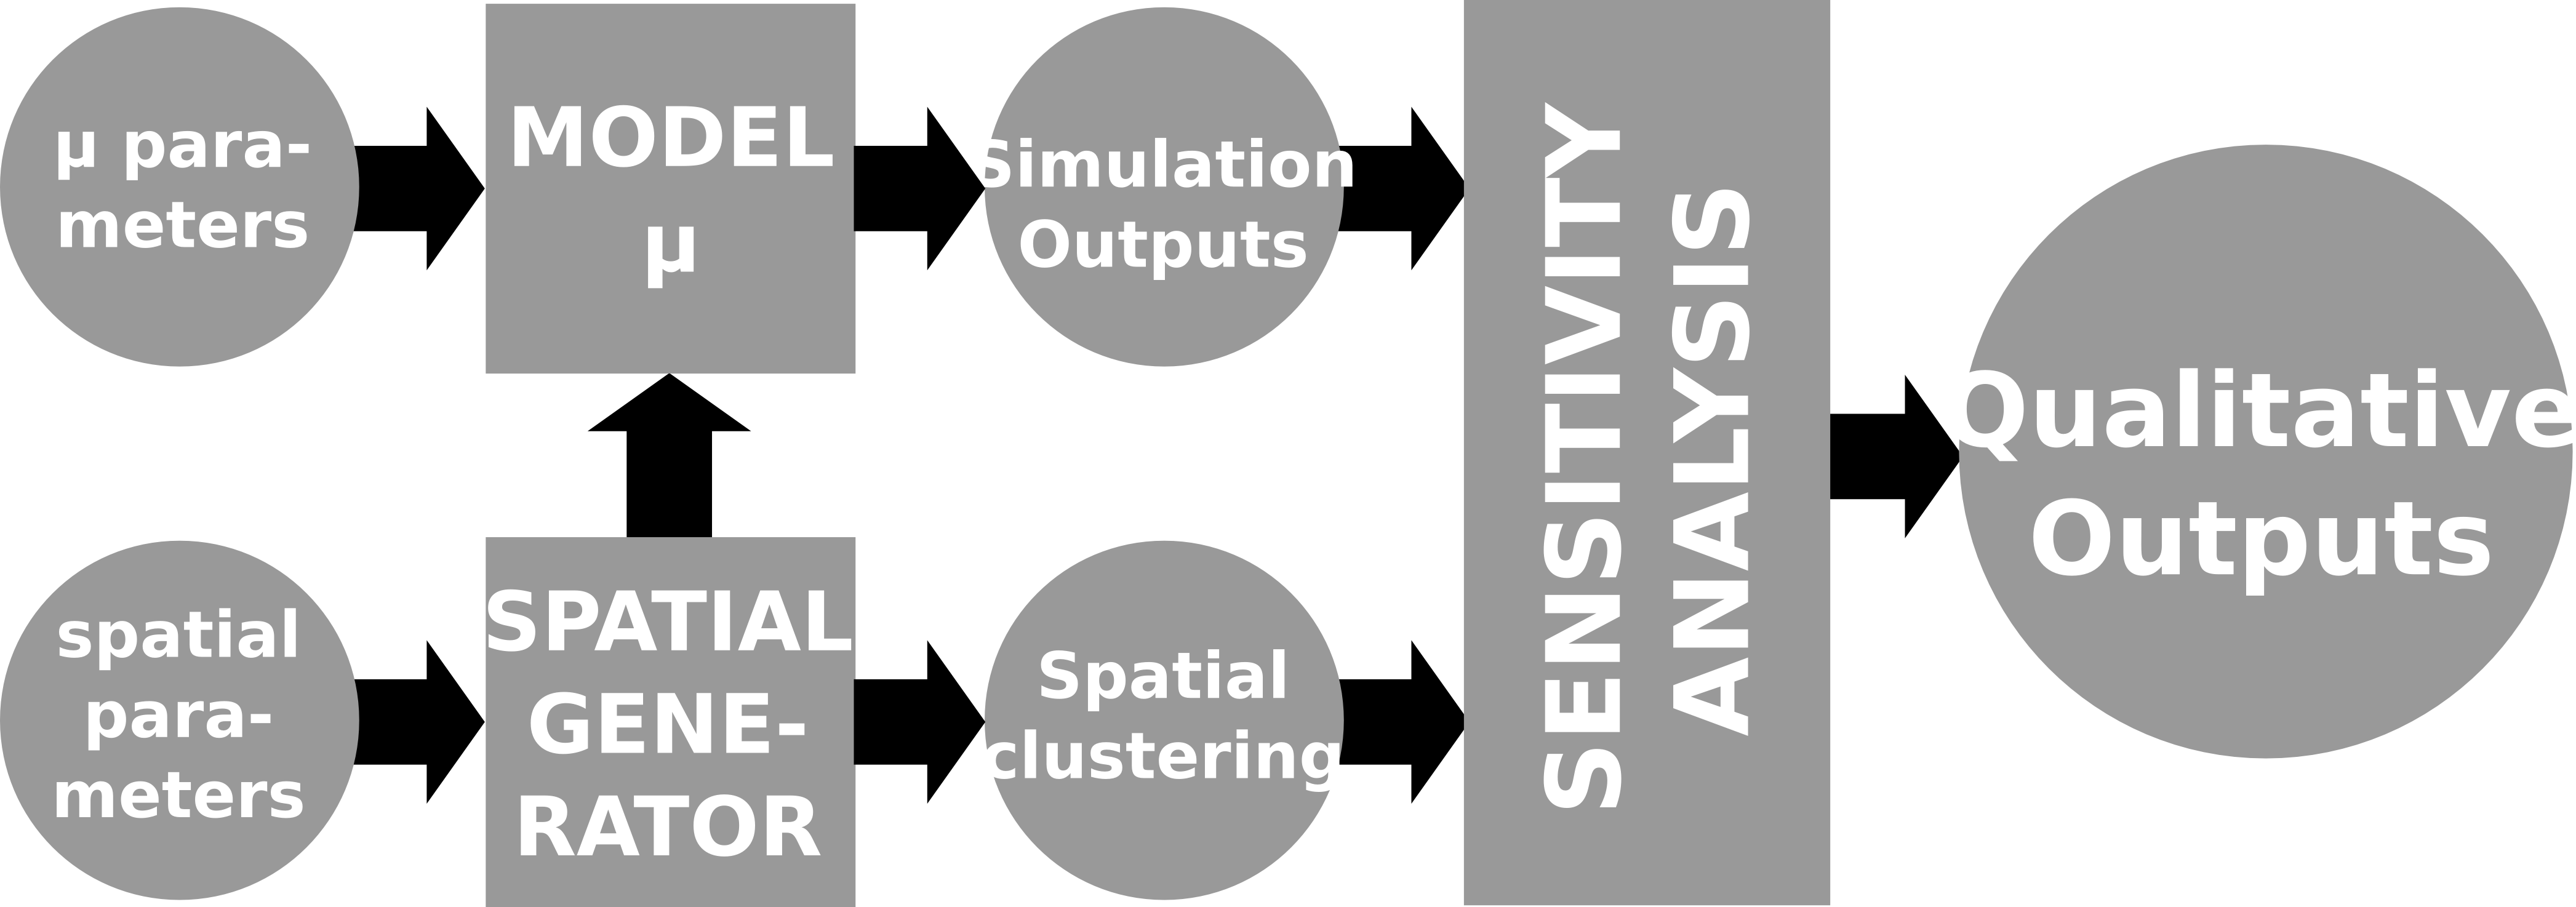
\includegraphics{figures/SchemaMeta_1.png}
} \caption{General workflow of our method\comment[MLT]{If we want to keep this figure, I propose that we link it more clearly to the following subsections, by numbering the different parts of the figure? By graphically showing on which parts of the figure the different subsections focus? Besides, we need to change it as we know want to go further than analysing the outputs qualitatively.}} \label{fig:method} \end{center} \end{figure*} %
%%%%%%%%%%%%%%%%%%%%%%





%%%%%%%%%%%%%%%%%%%%%%
\subsection{Constructing a spatial generator}

Our spatial generator applies an urban morphogenesis model (\cite{Batty2007}), which has been generalised, explored and calibrated (\cite{Raimbault2014}). In a nutshell, grids are generated through an iterative process which adds a quantity $N$ (population) at each time step, allocating it through preferential attachment characterised by its strength of attraction $\alpha$. This first growth process is then smoothed $n$ times using a diffusion process of strength $\beta$. Grids are thus generated from the combination of the values of these four meta-parameters $\alpha$, $\beta$, $n$ and $N$, in addition to the random seed. To ease our exploration, only the distribution of density is allowed to vary rather than the size of the grid, which we fix to a 50x50 square environment of 100,000 units (cf. figure \ref{fig:spatialGen}).


%%%%%%%%%%%%%%%%%%%%%%
\begin{figure*}[htbp] \begin{center} 
\resizebox{0.9\textwidth}{!}{ 
	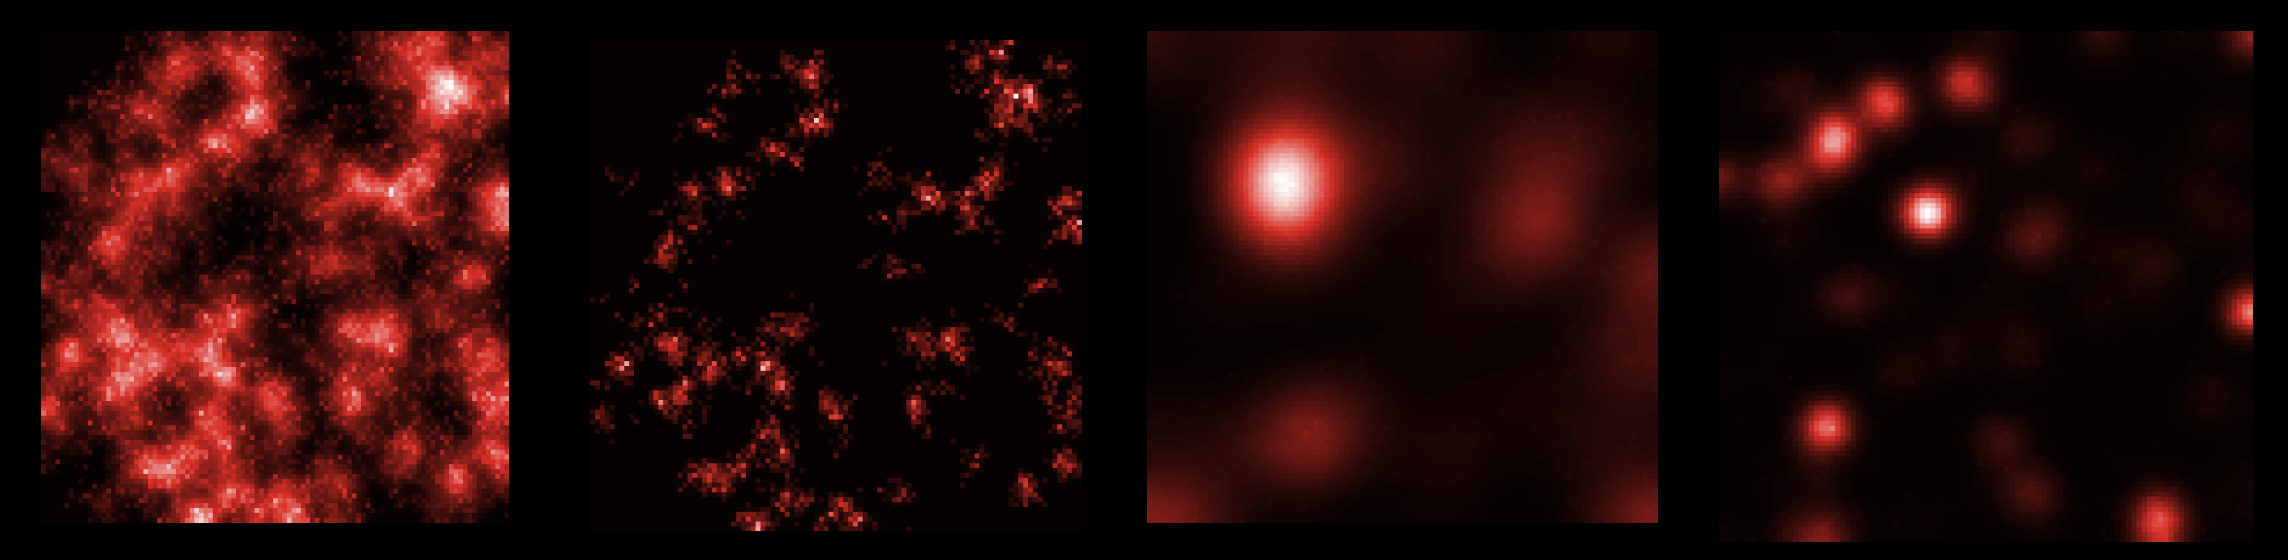
\includegraphics{figures/spatialGen.png}
} \caption{Four examples of grids produced by the spatial generator} \label{fig:spatialGen} \end{center} \end{figure*} %
%%%%%%%%%%%%%%%%%%%%%%


%%%%%%%%%%%%%%%%%%%%%%
\subsection{Including a (typical) variety of initial conditions in the sensitivity analysis}

In order to generate density grids which correspond to empirical density distributions, we select among the generated grids using an objective function which matches the point cloud of 110 metropolitan areas in Europe described by four dimensions: their concentration index, hierarchy index, centrality index and continuity index (cf. \cite{LeNechet2015}). A stochastic exploration of a Latin Hypercube Sampling of 2000 points in the 4-dimensional space of parameters {$\alpha$, $\beta$, $n$, $N$} gives a subset of 170 interesting grids matching empirical densities, which constituted our set of different initial spatial conditions. These are further clustered into three classes of morphology: compact (e.g. Vienna), polycentric (Liege) and discontinuous (Augsburg) in order to evaluate the non-trivial effects of urban form on simulation results. We select 15 grids of each type to work with.

%cite{Gauvinetal2009}


%%%%%%%%%%%%%%%%%%%%%%
\subsection{Comparing Phase Diagrams}

Problem: we have as many phase diagrams than we have spatial grids, so we cannot define the phases qualitatively. We need quantitative procedures.

Potential methods to explore: anisotropic spatial segregation index (number of clusters found and where in the parameter spaces? but may be weak...), earth Movers Distance (i.e. distance between probability distributions), comparison of transition matrices of the dynamic associated to the potential...
See also: http://mck.riks.nl/ to get some ideas.

A simple measure of the distance between two phase diagrams, relative to their internal variability, is given by

\[
d_r\left(\alpha_1,\alpha_2\right) = 2 \cdot \frac{d(f_{\vec{\alpha_1}},f_{\vec{\alpha_2}})}{Var\left[f_{\vec{\alpha_1}}\right] + Var\left[f_{\vec{\alpha_2}}\right]}
\]

where $f_{\vec{\alpha}}\left[\vec{x}\right]$ the operator giving phase diagrams with $\vec{x}$ parameters and $\vec{\alpha}$ meta-parameters, and $d$ is a functional distance that can be taken for example as basic L2 distance or the Earth's Mover Distance.

\todo[JR]{explain this in clear words}



%%%%%%%%%%%%%%%%%%%%%%
\section{Application cases}
%%%%%%%%%%%%%%%%%%%%%%

We use our set of initial density grids in two spatial simulation models: Schelling and Sugarscape.


%%%%%%%%%%%%%%%%%%%%%%
\subsection{Schelling's model of residential segregation}

Schelling's model consists in a abstract urban housing market where agents of different nature sense their environment, evaluate their satisfaction in terms of neighbourhood composition, and relocate if unsatisfied. It has been shown by \cite{Schelling1969} that even tolerant agents tended to produce segregated patterns because of the complexity of their local interactions. The main parameters of this model are the tolerance level (\% of agents similar to {\it ego}), the scope of sensing and the percentage of vacant spaces in the housing market. In addition, we are interested in testing the impact of the spatial distribution of housing capacity in this project, using the generated grids.


%%%%%%%%%%%%%%%%%%%%%%
\subsection{Sugarscape model of resource extraction and population settlement}

Sugarscape is a model of resource extraction which simulates the unequal distribution of wealth within a heterogenous population (\cite{EpsteinAxtell1996}). Agents of different vision scopes and different metabolisms harvest a self-regenerating resource available heterogeneously in the initial landscape, they settle and collect this resource, which leads some of them to survive and others to perish. The main parameters of this model are the number of agents, their minimal and maximal resource. In addition, we are interested in testing the impact of the spatial distribution of the resource in this project, using the generated grids. The outcome of the model is measured as a phase diagram of an index of inequality for ressource distribution (Gini index). We extend the implementation with agents wealth distribution of~\cite{li2009netlogo}.


%%%%%%%%%%%%%%%%%%%%%%
\section{Results}
%%%%%%%%%%%%%%%%%%%%%%


\comment[JR]{for the plan of the results section, I think the best is to organize by application case.}

%%%%%%%%%%%%%%%%%%%%%%
\subsection{Schelling's model}

We proceed to 4,500,000 simulation runs of the Schelling model (1000 parameter combinations x 45 density grids x 100 replications), using OpenMOLE to distribute the computation, and apply segregation measures to characterise the results. We find that the different urban morphologies impact the parameter interaction patterns, and that polycentric and discontinuous cities appear systematically more segregated than compact cities in terms of dissimilarity and entropy index.

%%%%%%%%%%%%%%%%%%%%%%
\subsection{Sugarscape model}

For Sugarscape, 2,500,000 simulations (1000 parameter points x 50 density grids x 50 replications) allow us to show that the model is more sensitive to space than to its other parameters, both qualitatively and quantitatively: the amplitude of variations across density grids is larger than the amplitude in each phase diagram, and the behavior of phase diagram is qualitatively different in different regions of the morphological space.



%%%%%%%%%%%%%%%%%%%%%%
\section{Discussion}
%%%%%%%%%%%%%%%%%%%%%%



% \hfill \break
% \itshape{This is a sub, subheading}\normalfont

% \hfill\break

%
%
%\begin{table}[htp]
%
%\begin{center}
%\begin{tabular}{c c c c}
%\arrayrulecolor{black}
%\hline 
%This & Is & A & Table\\
%\arrayrulecolor{lightgray}
%\hline 
%\arrayrulecolor{black}
%Label & 0.1 & 0.2 & 0.3\\
%Label & 1.0 & 2.0 & 3.0\\
%\hline
%\end{tabular}
%\end{center}
%\label{first_table}
%\caption{This is a table caption}
%\end{table}%
%
%
%
%\begin{equation}
%a^2 + b^2 = c^2
%\tag*{Equation 1}
%\end{equation}

%%%%%%%%%%%%%
% Acknowledgements

\begin{acks}
The authors acknowledge the funding of their institutions and the EPSRC project number EP/M023583/1. Results obtained in this paper were computed on the vo.complex-system.eu virtual organization of the European Grid Infrastructure ( http://www.egi.eu ). We thank the European Grid Infrastructure and its supporting National Grid Initiatives (France-Grilles in particular) for providing the technical support and infrastructure.
\end{acks}




%%%%%%%%%%%%
%% References
%%%%%%%%%%%%


\bibliographystyle{SageH}
\bibliography{spacematters,biblio}


\end{document}
